\documentclass[sigconf]{acmart}

\usepackage{booktabs} % For formal tables
\usepackage{amsmath}
\usepackage[ruled,linesnumbered]{algorithm2e}
\SetKwComment{Comment}{$\triangleright$\ }{}
\usepackage{caption}
\usepackage{graphicx}
\usepackage[export]{adjustbox}
\settopmatter{printacmref=false}
\usepackage{subcaption}
\usepackage{bbm}
\usepackage{bm}
\usepackage{multirow}
% Copyright
%\setcopyright{none}
%\setcopyright{acmcopyright}
%\setcopyright{acmlicensed}
\setcopyright{rightsretained}
%\setcopyright{usgov}
%\setcopyright{usgovmixed}
%\setcopyright{cagov}
%\setcopyright{cagovmixed}


% DOI
\acmDOI{10.475/123_4}

% ISBN
\acmISBN{123-4567-24-567/08/06}

%Conference
\acmConference[WOODSTOCK'97]{ACM Woodstock conference}{July 1997}{El
  Paso, Texas USA}
\acmYear{1997}
\copyrightyear{2016}


\acmArticle{4}
\acmPrice{15.00}

% These commands are optional
%\acmBooktitle{Transactions of the ACM Woodstock conference}
\editor{Jennifer B. Sartor}
\editor{Theo D'Hondt}
\editor{Wolfgang De Meuter}


\begin{document}
\title{Convolutional Neural Networks for Identify Target Entity Types}
%\titlenote{Produces the permission block, and  copyright information}
%\subtitle{Extended Abstract}
%\subtitlenote{The full version of the author's guide is available as
%  \texttt{acmart.pdf} document}


%\author{Ben Trovato}
%\authornote{Dr.~Trovato insisted his name be first.}
%\orcid{1234-5678-9012}
%\affiliation{%
%  \institution{Institute for Clarity in Documentation}
%  \streetaddress{P.O. Box 1212}
%  \city{Dublin}
%  \state{Ohio}
%  \postcode{43017-6221}
%}
%\email{trovato@corporation.com}
%
%\author{G.K.M. Tobin}
%\authornote{The secretary disavows any knowledge of this author's actions.}
%\affiliation{%
%  \institution{Institute for Clarity in Documentation}
%  \streetaddress{P.O. Box 1212}
%  \city{Dublin}
%  \state{Ohio}
%  \postcode{43017-6221}
%}
%\email{webmaster@marysville-ohio.com}
%
%\author{Lars Th{\o}rv{\"a}ld}
%\authornote{This author is the
%  one who did all the really hard work.}
%\affiliation{%
%  \institution{The Th{\o}rv{\"a}ld Group}
%  \streetaddress{1 Th{\o}rv{\"a}ld Circle}
%  \city{Hekla}
%  \country{Iceland}}
%\email{larst@affiliation.org}
%
%
%\author{Julius P.~Kumquat}
%\affiliation{\institution{The Kumquat Consortium}}
%\email{jpkumquat@consortium.net}
%
%% The default list of authors is too long for headers.
%\renewcommand{\shortauthors}{B. Trovato et al.}


\begin{abstract}
Identifying the target type of entity bearing queries can help improve the overall performance of the search. In this work, we propose a deep neural network approach to solve the problem. The main benefit of this approach is that it is not necessary to provide hand-made features to the network. The main contribution of this paper is to use CNN networks, to extract different aspect of importance in target type identification problem. We show our approach outperforms the existing LTR approach by a remarkable margin.
\end{abstract}

%
% The code below should be generated by the tool at
% http://dl.acm.org/ccs.cfm
% Please copy and paste the code instead of the example below.
%



\keywords{Query understanding, query types, entity search, neural network, deep learning}


\maketitle



\section{Introduction}\label{introduction}
\par
A large portion of queries in web search is related to entity retrieval, each entity has a specific type which can be mapped to hierarchical structure i.e taxonomy. General knowledge bases such as Wikipedia provide such taxonomies. In recent years, commercial search engines answer the entity bearing queries using entity cards \cite{}. Entity cards summarize the information need of the user and he/she can find the answer in the search page. It can enhance the user experience and reduce search session time. Accordingly, research in entity retrieval has been an important topic in the IR community in recent years.
\par
In order to enhance the quality of entity retrieval, several solutions e.g target type identification \cite{}, attribute detection \cite{} has been proposed. In target type identification problem,  given a query, the goal is to identify the type of relevant result with respect to a given ontology. Previous research indicates that automatic target type identification can improve the precision of retrieval without complicating the user interface (i.e single search box). Target identification can enhance the performance of retrieval in both web search and product search \cite{}.
\par
The previous research for type retrieval problem, can be divided into two categories i.e probabilistic and learning to rank (LTR) models. Although the LTR model has better performance in comparison with the probabilistic model but the LTR model needs several hand-crafted domain-wise features which restrict the usage of such model in cross domains.

Here in this paper, our motivation is to provide a suitable neural network structure which can learn important features in automatic type identification problem.

Our observation in this research indicates that a simple feed forward neural network can not solve the problem efficiently. Therefore in this paper, we propose a convolution neural network to capture important features of this problem. 

According to previous research, we use type centric (TC) and entity centric (EC) approaches to propose the architecture of the neural network. This research indicates that each of these approaches captures a different aspect of query and type matching and therefore a single model which combine these models has better performance.

The main contribution of this paper is to use a CNN network to capture the importancy of words (i.e features) in the context of the given query, both in entity and type centric models. the proposed model outperforms the probabilistic model by high margin and works slightly worse than the LTR although without any hand-crafted features.

\section{Problem Spec and Related Work}
In this section, we first define the problem of Target Identification problem and then we propose the state-of-the-art approaches for solving this problem.

\subsection{Problem Definition}
Here the objective is to assign target types to queries from a type taxonomy. more formally we borrow the definition of the task from \cite{} :

"Find the main target types of a query, from a type taxonomy, such that (i) these correspond to the most specific category of entities that are relevant to the query, and (ii) main types cannot be on the same path in the taxonomy. If no matching type can be found in the taxonomy then the query is assigned a special NIL-type."

\subsection{Entity Centric (EC)}\label{EC}
The idea of this method is to rank entities based on their relevance to the query, then according to the top-k ranked entities, the target type of query will be determined. This model is similar to late fusion design pattern for object retrieval \cite{22Hasibi} in which the relevance scores of each type is determined as follows:
\begin{equation}
score_{EC}(t,q) = \sum_{e\in R_K(q)}{score(q,e)\times W(e,t)}
\end{equation}
Where $R_k$ is the set of top-k ranked entities for query $q$ and $score(q,e)$ indicates retrieval score of entity $e$ based on language model with Dirichlet smoothing (k=2000). The entity-type association weight, $W(e,t)$ is set uniformly across entities that are typed with $t$, i.e., $W(e,t)=1/\sum_{e^\prime}{\mathbbm{1}(e^\prime,t)}$, and is 0 otherwise.
$\mathbbm{1}(e,t)$ is an indicator function that returns $1$ if $e$ is typed with $t$, otherwise returns $0$.

\subsection{Type Centric (TC)}
In this method by aggregating descriptions of entities of a specific type, a pseudo document is generated for that type and these documents will be use in ranking. This method is refer to as the early fusion design pattern for object retrieval in \cite{22hasibi}. The pseudo frequency of a word for a type is defined as 
$\tilde{f}(w,t) = \sum_{e}{f(w,e)\times w(e,t)}$, where $f(w,e)$ is the frequency of the term $w$ in (the description of) entity $e$ and $w(e,t)$, as before, denotes the entity-type association weight. The relevance score of a type for a given query $q$ is then calculated as the sum of the individual query term scores:
\begin{equation}
score_{TC}(t,q) = \sum_{i=1}^{|q|}{score_{LM}(q_i,\tilde{f})}
\end{equation}
where $score_{LM}(q_i,\tilde{f})$ is the retrieval score of pseudo document of $t$. We use the same parameter settings as in \ref{EC}.

\subsection{Learning to Rank (LTR)}
The entity and type centric models capture different aspect of the task and the learning to rank approach proposed in \cite{hasibiSig17} combined these two models in a single framework. In this approach three main feature categories have been used to combine several ranking signals as follows:
\begin{enumerate}
	\item \textit{TC and EC features}: this category includes five features which measure the relevancy of query and type based on EC and TC approaches.
	\item \textit{Knowledge base features}: this category includes four features which indicate the properties of the target type in taxonomy (e.g depth, number of children type, etc.).
	\item \textit{Type label features}: this category includes eight features which capture the properties of target type (e.g length of type $t$ in words, etc.)
\end{enumerate}
They employed a random forest algorithm for regression as the supervised ranking method. their propose LTR model outperforms EC and TC methods by a remarkable margin but the main problem with this approach is that the features are related to the domain of problem and it can not be easily generalize to other domains such as e-commerce search engines.

\section{Our Approach}
Our motivation in this paper is to propose a method with minimal feature engineering effort to solve target type identification. For this task, we use the test collection introduce in \cite{hasibiSig17}. In this test collection, for a given query there is a pool of target entity types. for each target type in the pool, there is a label between zero (non-relevant) and seven (the most relevant) which indicate the relevance degree of the query and that target type. Similar to the propose LTR approach in \cite{hasibiSig17} we cast the type identification problem into regression problem i.e for a given pair of query and type the goal is to predict the relevancy score.

Following the idea of TC and EC method introduce in \label{key} we defined two matrices i.e $I_{TC}$ and $I_{EC}$ that models word level similarities via word embeddings. 

\boldsymbol{$I_{TC}:$} For a given query-type pair $(q,t)$, we first extract top-50 words representing type $t$. These words are selected according to the tf.idf score. We then build $I_{TC}$ matrix as follows. Each row of matrix indicates a query term (e.g $q_i$) of $q$ (in order of occurrence) and each column of the matrix indicates a representing word (e.g $w_j$) of that type (sorted by tf.idf score). The entry $I_{TC}[i,j] = cos(\vec{q_i}, \vec{w_j})$ where $\vec{q_i}$ and $\vec{w_j}$ indicates the pre-trained word embedding vectors of \cite{mikolovGoogle16Hasibi}.

\boldsymbol{$I_{EC}:$} For a given query-type pair $(q,t)$, we first used a language retrieval model to retrieve top-20 ranked entities (i.e $e_1,\cdots, e_{20}$) for query $q$. $I_{EC}$ is made by concatenation of twenty matrices as $I_{EC} = [I_{E_1C},\cdots, I_{E_{20}C}]$ where $I_{E_iC}$ is a matrix indicating the relevancy of query $q$ and entity $e_i$ considering the type $t$. Each entry of matrix $I_{E_iC}$ is computed as follows:
\begin{equation}
I_{E_iC}[m,n] = 
\begin{cases}
cos(q_m,w_{i,n}) \times W(e,t) &\quad\text{type(e)} \cap t \neq \phi \\
0 &\quad\text{otherwise} \\
\end{cases}
\end{equation}
Where $q_m$ is the $m^{\text{\tiny th}}$ query term and $w_{i,n}$ ($1\leq n \leq20$) indicates the $n^{\text{\tiny th}}$ word (sorted on tf.idf score) representing the entity $e_i$. $W(e,t)$ is the function  described in section \ref{EC} and $type(e)$ is the set of types associate with entity $e$.


In our first attempt to solve the problem we use two feedforward neural networks. the input of these networks are $I_{TC}$ and $I_{EC}$, respectively. the number of layers and neurons are indicated in table X.


Similar to the translation, rotation and scale invariance of images in CNN, CNN is able to learn the local features from words or phrases in different places of text \cite{aclweb}. As a result, in our second attempt, we present a jointed convolutional neural network and feedforward (FF) architecture that takes the local features extracted by CNN as input to FF for target type identification problem. We try this architecture twice with $I_{EC}$ and $I_{TC}$ as the inputs of the CNN models, respectively. The detail of each network is indicated in table X.

Finally, following the idea of combining entity centric and type centric models\cite{cikmBalog,SigHasibi}, we propose the architecture represented in \textbf{fig.X}. This architecture is the combination of the above mentioned CNN+FF networks.


\section{Model Implementation Details}
This section describes the configuration of the FF and CNN+FF Models.

\textbf{Model Training} is performed using 5 fold\textit{nested cross-validation} \cite{Nested } where model hyperparameters are selected for each test fold based on standard CV experiments on the training folds. The hyperparameters of the models are indicated in table x.

\textbf{Model Optimization} use the adam optimizer with batch size 128, learning rate 0.0001 and $\epsilon$ X. We implemented our model using Keras \cite{kerasCite}.

\textbf{Model Structure} model structure of CNN+FF is depicted in fig.X. The feedforward model of type centric approach is a three-layer network with [1000, 1000, 5000] neurons. The activation function is relu. the dropout parameter is selected to be 0.3. The feedforward model of entity centric approach is a one-layer network with 1000 neurons. The activation function is relu. the dropout parameter is selected to be 0.


\section{Result And Discussion}
Table X presents the evaluation results. We find that the feedforward network significantly (except Entity Centric for NDCG@5 measure) outperform the probabilistic model both in the entity and type centric approaches. significantly improvement is measured with $p$<0.001 using two-tailed pair-test. In addition, the CNN+FF architecture improves the feedforward network significantly by a large margin both in entity centric and type centric approaches. Another interesting observation here is that the hybrid model (i.e entity + type centric) can improve the NDCG@1 and NDCG@5 significantly.

The interesting observation here is that the NDCG@1 of CNN+FF model (in hybrid setting) is not worse than the LTR model significantly. In other words, although, the LTR model utilizes several hand-crafted features, it can not outperform the CNN+FF propose model.

In order to better analyze the behavior of CNN network, we visualize the input of $I_{TC}$ and the output of first convolution layer for the query \textit{"Give me a list of all trumpet players that were bandleaders."} and type \textit{"MusicalArtist"} in fig1.a and fig1.b respectively. As indicated in these figures the horizontal axis indicates top-50 words representing \textit{MusicalArtist} type sorted by tf.idf from left to right. in this figure, lighter entries indicate the larger value of similarity between a query term and the corresponding representing term. By comparing the output and output matrices, we find that the CNN model is able to remove noises i.e non-relevant terms to that specific type. for example the weights associated with query terms "\textit{give}" and "\textit{me}" are reduced significantly. According to this observation, CNN network outperforms the FF because it can extract local features (by local we means the feature associated with the context of query) while the FF network only uses the word2vec embedding of each word and that not consider it's context in the query. our proposed model is an economic model because we don't use any complicated features, but it can capture the relationship between the query and it's target type effectively.     

\begin{figure*}
	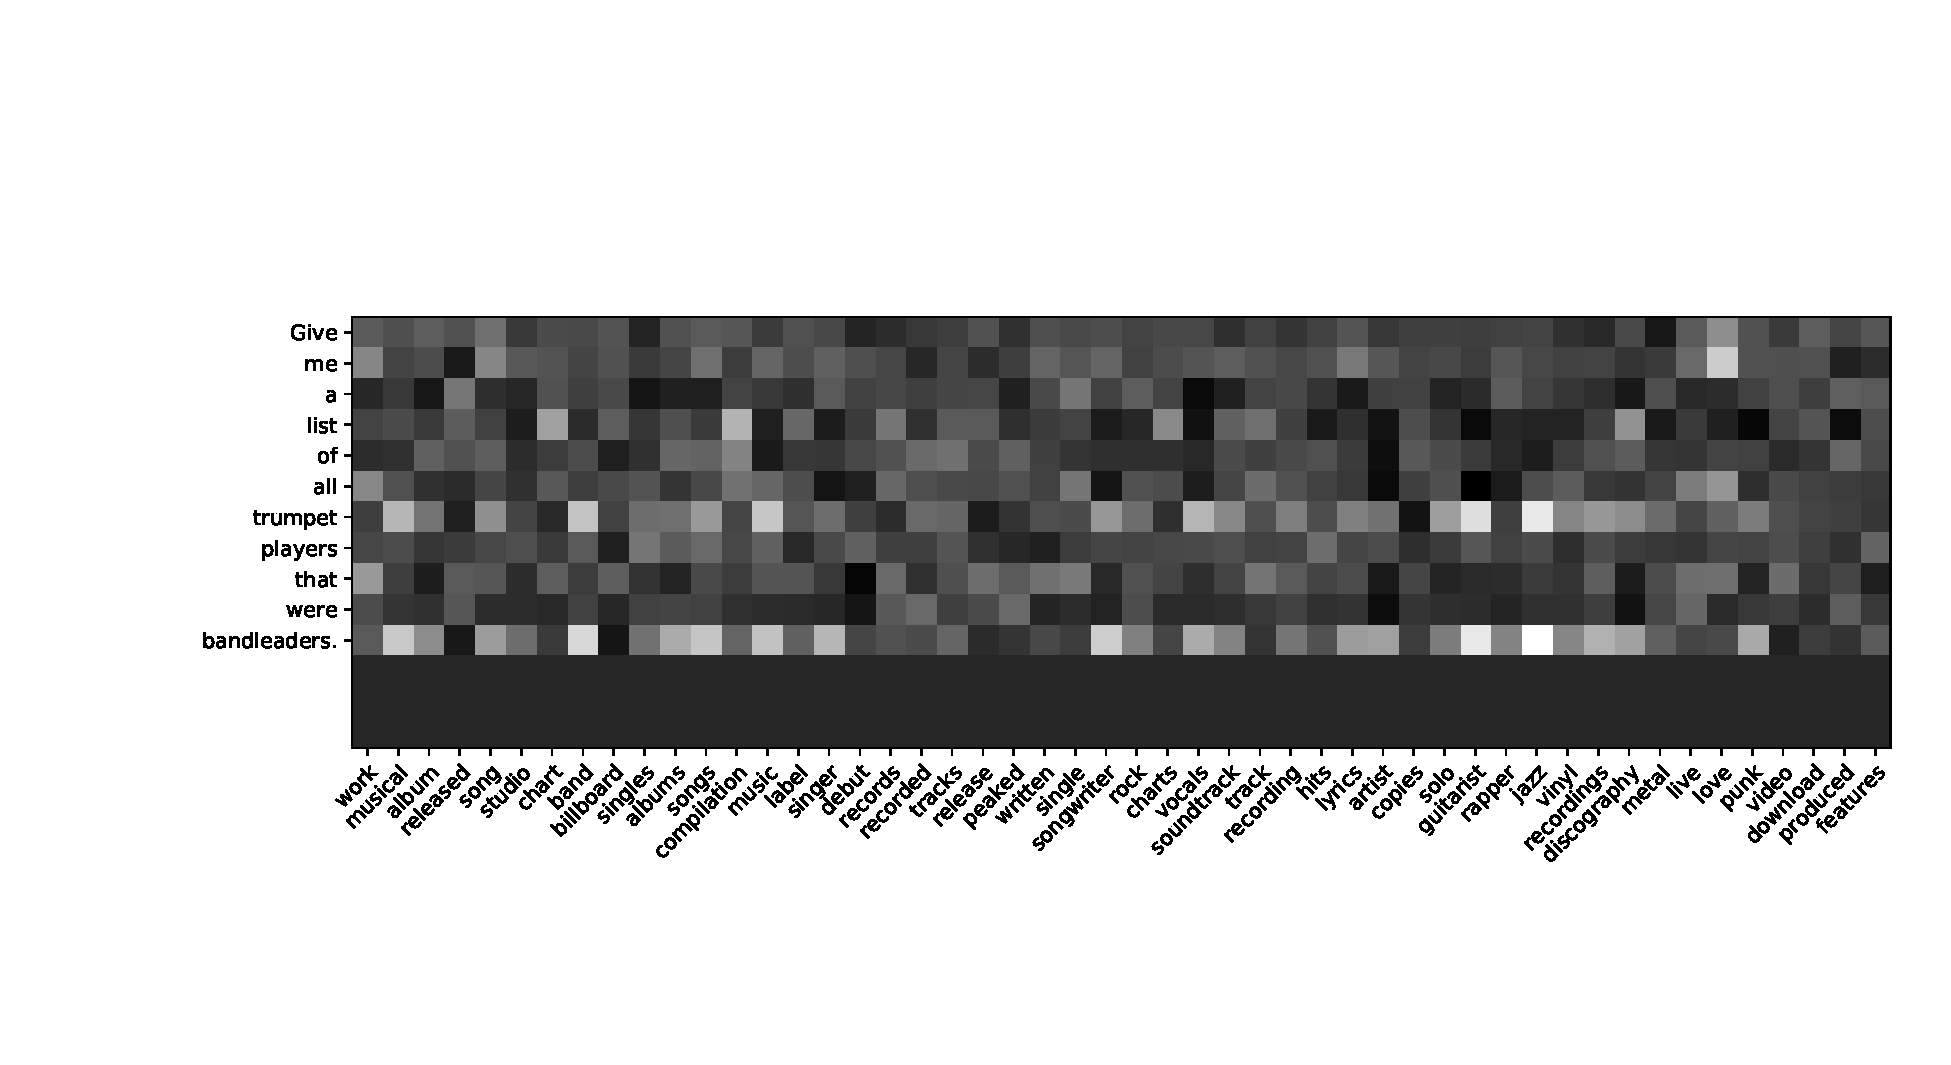
\includegraphics[width=\textwidth]{leaders_input.pdf}
	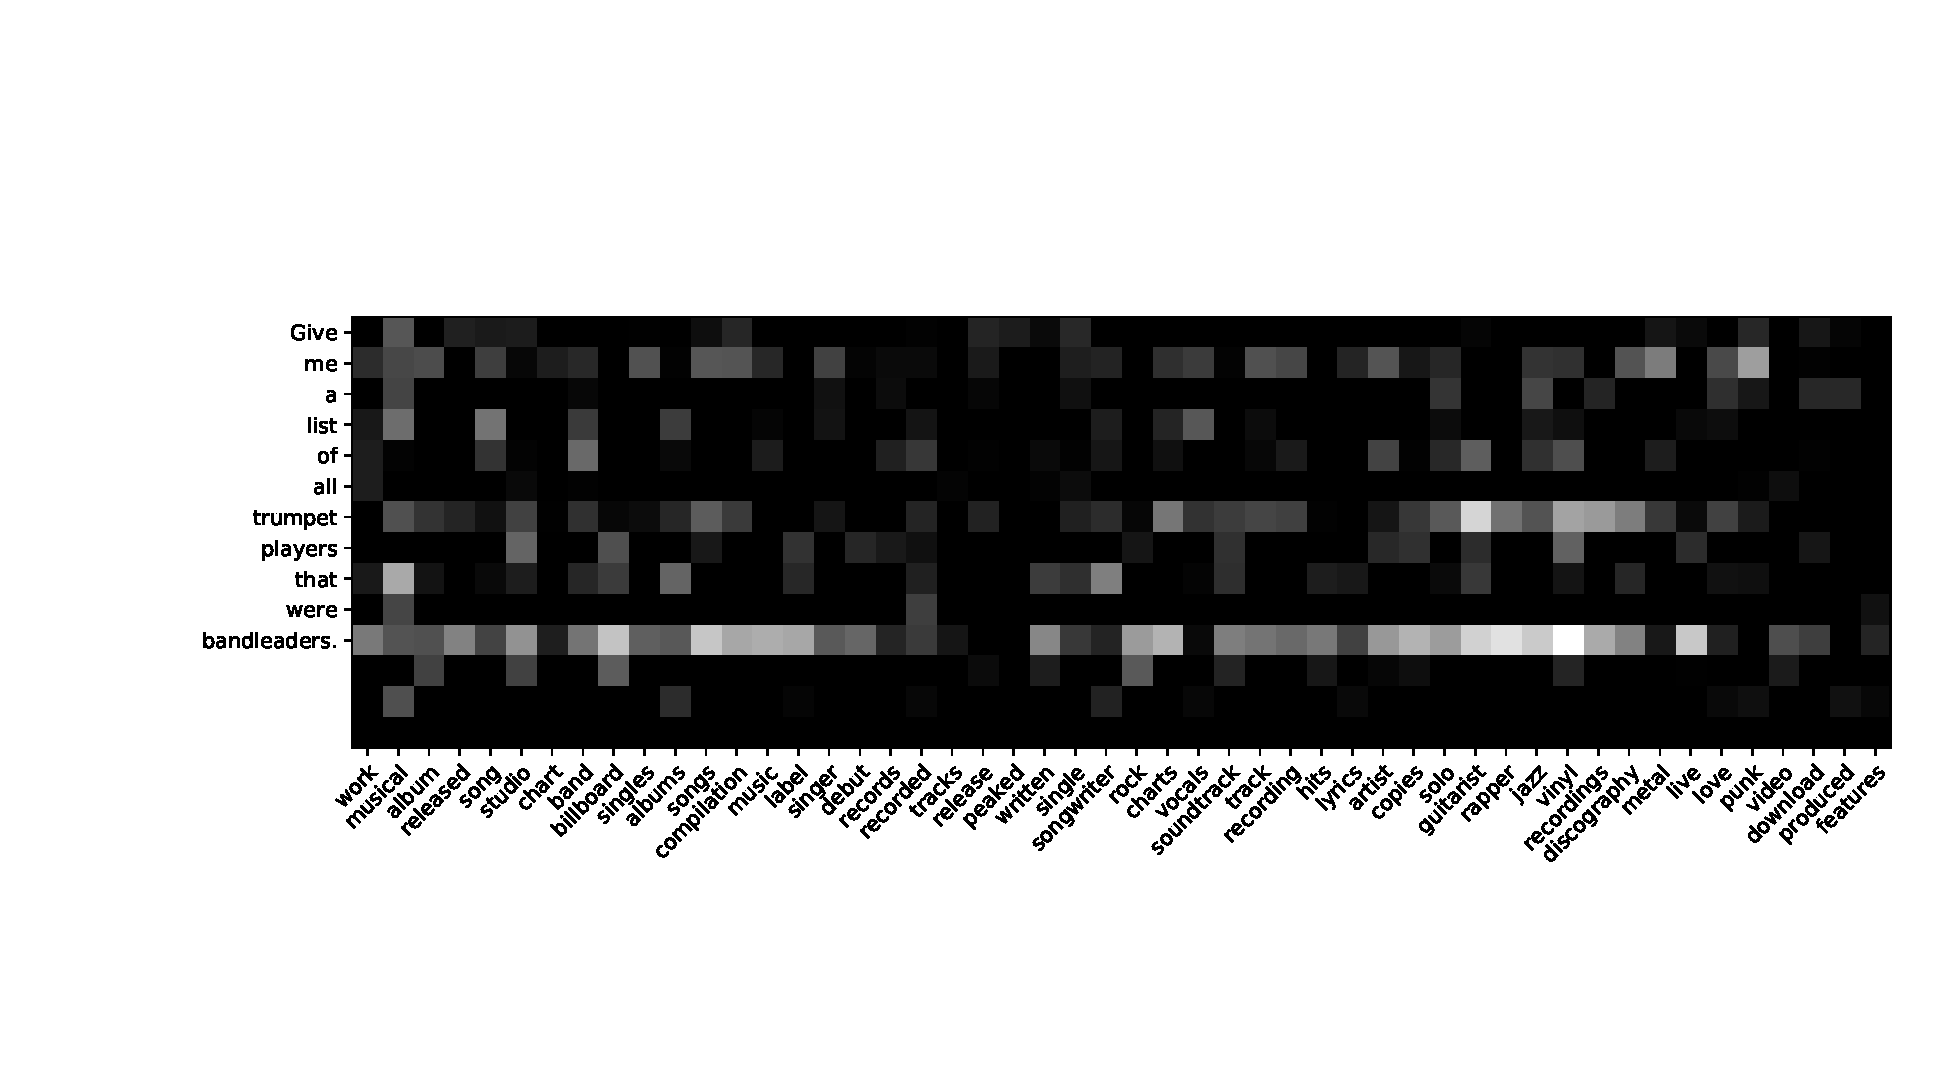
\includegraphics[width=\textwidth]{leaders_out.pdf}
	\caption{This is a figure caption}
\end{figure*}



% Please add the following required packages to your document preamble:
% \usepackage{multirow}
% Please add the following required packages to your document preamble:
% \usepackage{multirow}
\begin{table}[]
	\begin{tabular}{c|c|c|c}
		
		Feature Group                               & Retrieval model                & NDCG@1   & NDCG@5   \\ \hline
		Entity Centric                              & \multirow{2}{*}{Probabilistic} & 0.1490   & 0.3223   \\ 
		Type Centric                                &                                & 0.2341   & 0.3780   \\ \hline
		Entity Centric                              & \multirow{2}{*}{Feed Forward}  & 0.1886*  & 0.3289   \\ 
		Type Centric                                &                                & 0.2786*  & 0.4011*  \\ \hline
		Entity Centric                              & \multirow{2}{*}{CNN + FF}      & 0.3341** & 0.4586** \\ 
		Type Centric                                &                                & 0.4034** & 0.5287** \\ \hline
		Entity + Type                               & CNN + FF                       & 0.4575   & 0.5994   \\ \hline
		Entity + Type + Knowledge Base + Type Label & LTR                            & 0.4842   & 0.6355   \\ \hline
	\end{tabular}
\end{table}



\bibliographystyle{ACM-Reference-Format}
\bibliography{bibliography}


\end{document}
